\def\year{2020}\relax

\documentclass[letterpaper]{article} %DO NOT CHANGE THIS
\usepackage{aaai20}  %Required
\usepackage{times}  %Required
\usepackage{helvet}  %Required
\usepackage{courier}  %Required
\usepackage{url}  %Required
\usepackage{graphicx}  %Required
\frenchspacing  %Required
\setlength{\pdfpagewidth}{8.5in}  %Required
\setlength{\pdfpageheight}{11in}  %Required
\setcounter{secnumdepth}{0}  
\usepackage{subfigure}

\begin{document}
% The file aaai.sty is the style file for AAAI Press 
% proceedings, working notes, and technical reports.
%
\title{Sentiment Analysis of COVID-19 Social Distancing Tweets}
\author{Jian Sun, Diwen Zhu, Zihao Di\\
\{j248sun ,d55zhu , z2di\}@uwaterloo.ca\\
University of Waterloo\\
Waterloo, ON, Canada\\
}
\maketitle


%%%%%%%%% Introduction %%%%%%%%%

\section{Introduction}

This paper describes an artificial intelligence platform for sentiment analysis on Covid-19 related Tweets in Canada and the United States. The Tweets will be classified into two sentiment categories: positive and negative. The goal is to build and train a neural networks classifier to gauge public opinion on social distancing orders in real time. This project will seek to analyze the prediction accuracy of a LSTM-CNN ensemble model trained on a general Tweets dataset and evaluated on a dataset of Covid-19 Tweets. Having knowledge of public sentiment on Covid-19 could help local authorities improve and adjust their social distancing policies to better suit the needs of the public in a timely manner.

Twitter is a social networking platform that allows users to post messages called Tweets with a limit of 280 characters. Twitter has two main components: a user timeline that shows Tweets sent by a particular user and a home timeline which displays Tweets of users that a user follows.

As the Covid-19 pandemic continues to develop around the world, governments have started to implement strict social distancing orders in order to curb the spread of the virus. The implementation of these measures, however, are accompanied by many problems: some have reported they are unable to get essential supplies because of the lack of transportation options while others say the lack of social interactions is taking a heavy toll on their mental health (Breen 2020).

The real-world impact of this project is its ability to allow local authorities, government officials and decision makers in the healthcare industry to better understand the public opinions on the implemented measures in real time. This information can be used to make adjustments and improvements to the measures, which will make social distancing more effective in combating the pandemic. For example, if sentiment in an area is overwhelmingly negative, authorities can immediately investigate and see if social distancing is causing unintended problems for some. After making changes to their policy, authorities can continue to monitor sentiment levels to see whether it improves, which helps them determine whether these changes are effective.

%%%%%%%%% Summary of your contributions %%%%%%%%%

\section{Contributions}
Much of the prior machine learning research done on Twitter sentiment analysis focuses on training a model on a generic set of Tweets and evaluating its accuracy on another generic set of Tweets. Covid-19 Tweets are very specific and may contain patterns and sentence structures not found in generic Tweets. This paper seeks to answer the research question: given a LSTM-CNN model trained using a generic set of Tweets, is there a significant difference in prediction accuracy when this model is evaluated on a set of Covid-19 Tweets? If so, can the model's parameters be tuned to improve its accuracy?

The training and evaluation procedures utilizes Sosa (2017)'s implementations. The model to be used is an ensemble of Long-Short Term Memory (LSTM) and Convolutional Neural Network (CNN).  The input words in each Tweet is first encoded by the LSTM layer, which stores patterns of both the current and the previous inputs. This encoding is then fed directly into a CNN layer, which recognizes local patterns within the text. The output of the CNN is then reduced to produce either positive or negative labels (Sosa 2017). The training process uses the Adam algorithm (a variation of gradient descent), the cross-entropy loss function, and the ReLu activation function. A dataset of 1.6 million generic Tweets with an even distribution of positive and negative sentiments will be used to train the model. A set of 10,000 Covid-19 specific Tweets with a real-world distribution of sentiments will be used to evaluate the model. 

The evaluation procedure has already been implemented by Sosa along with the training code. Sosa's implementation leverages TensorFlow's built-in functions to evaluate the cross-entropy loss and accuracy of the model at certain intervals during the training process. An overall summary of the model's training loss and accuracy is produced after training by the program automatically. The loss and accuracy of the model will also be evaluated when the model is used to make predictions on the evaluation dataset.

Without parameter tuning, the accuracy of the model is expected to be worse than Sosa's (2017) 75.2\% accuracy due to the specificity in structure and complexity of Covid-19 Tweets. However, the accuracy of the model should improve with additional parameter tuning.


%%%%%%%%% Related Work %%%%%%%%%

\section{Related Work}

Since 2001, there has been an explosive growth in sentiment analysis research due to the development of machine learning techniques and the wide availability of datasets (Pang \& Lee, 2008). With the rise of microblogging platforms such as Twitter in recent years, researchers have begun to develop better sentence-level analysis techniques instead of reusing those that analyze large opinionated pieces such as product reviews (Kim \& Hovy 2004). These generally don't seem to work well with texts that are more expressive and less structured, such as Tweets (Zhang et al. 2011). 

Most of the research in the area of sentence-level analysis is either lexicon-based or machine learning-based. The lexicon-based approach uses a precompiled list of opinion words to detect sentiment (Kim \& Hovy 2004). However, when applied to sentence-level analysis, this approach can result in low recall (Zhang et al. 2011; Wan \& Gao 2015). The machine learning-based approach generally uses supervised learning methods to train classifier models and requires labeled datasets (Zhang et al. 2011; Wan \& Gao 2015; Sosa 2017).

One paper from Wan \& Gao (2015) proposes an ensemble method that combines five separately trained machine learning models including Naive Bayesian, Bayesian Network, SVM, Decision Tree, and Random Forest. Although this combined approach outperforms each of the five models individually with an accuracy of 84.2\%, it is only 0.5\% higher than that of the runner-up, C4.5 Decision Tree which has an accuracy of 83.7\%. Furthermore, this method uses the majority vote of the five models with equal weighting to make its final decision, which may not be optimal as some of the models are more accurate than others individually.

Another idea proposed by Sosa (2017) combines Long-short Term Memory Neural Networks (LSTM) and Convolutional Neural Networks (CNN). In this combined approach, LSTM encodes the input tokens while maintaining information of all previous tokens, and CNN finds patterns using the richer encoded input. By taking advantage of both methods, the LSTM-CNN achieves an accuracy of 75.2\% which is better than either LSTM (72.5\%) or CNN (66.7\%) individually. The results from a similar approach taken by Severyn \&  Moschitti  (2015) using deep convolutional neural networks also produces similar results.

The approach used in this paper builds on the idea proposed by Sosa (2017). A LSTM-CNN model will be trained using a generic set of Tweets and evaluated on a set of Covid-19 Tweets. This project seeks to achieve comparable accuracy to Sosa's results by tuning the parameters of the model.


%%%%%%%%% Methodology %%%%%%%%%

\section{Methodology}
\subsection{Evaluation Method}

A generic Tweets dataset and a Covid-19 specific dataset will be used to train and evaluate the model, respectively. The generic dataset is from Kaggle and contains 1,600,000 Tweets with sentiment labels (Anova 2017) and an even distribution of positive and negative sentiments. The sentiment labels for this dataset were created by looking at positive and negative emoticons in each Tweet such as ":)" and ":(". This dataset was chosen because it contains a large amount of data points, is evenly split between positive and negative sentiments which could improve training accuracy (Sosa 2017), and is already pre-populated with Tweet text and labels. A pre-processing step must be done to remove any non-ASCII characters, such as Japanese characters, from the dataset to reduce noise for the training algorithm. 

The Covid-19 specific Tweets will be created by querying Twitter for English Tweets containing the keywords "social distancing $<$positive emoticons$>$ OR $<$negative emoticons$>$" between February and May 2020 within Canada and the United States. Sentiment labels will be added using a similar method as the Kaggle dataset by leveraging positive and negative emoticons. A target of 10,000 Tweets will be fetched. This is a reasonable method because sentiment labelling is consistent with the training dataset, and the results of this Twitter query contains a real-world distribution of positive and negative sentiments.

Using the Sosa's (2017) evaluation method, the trained model is to be evaluated on the labelled Covid-19 dataset. The evaluation process will yield two values: the accuracy of the model, which is the percentage of correctly classified Tweets, and a cross-entropy loss value. The cross-entropy loss function is used for both training and evaluation because it punishes misclassifications more than the mean squared error function, and therefore is better suited for classification problems. This is a reasonable way to evaluate the model because the Covid-19 dataset is never used in training and therefore never seen by the model, so the results will reflect the true accuracy of the model.

It will take one week to download and pre-process the generic and Covid-19 raw datasets. The evaluation implementation is already done by Sosa, so the evaluation will be done alongside the training and parameter tuning for 3-4 weeks afterwards. 

\subsection{Algorithms}

The chosen algorithm is the LSTM-CNN ensemble model proposed by Sosa (2017), shown in figure 1.  The LSTM-CNN ensemble model is appropriate for answering the research question because it has a number of distinct advantages over other algorithms. Neural networks are good at processing large amounts of non-tabular text data. It is also not appropriate to represent Tweet text classification using an if-else-then function as in decision trees. Furthermore, the complex nature of the ensemble neural networks model allows it to better understand the various intricate structures and patterns in human language than decision trees. Neural networks are also a better choice than Bayesian networks for this task. In sentiment classification, features are usually the n-gram of the input text data, which violates the Bayesian assumption of independence as neighboring n-grams will always overlap along the sequence (Aggarwal \& Reddy 2014). However, being able to analyze n-grams is beneficial because they carry more information per unit than unigrams (Wan \& Gao 2015). Finally, Bayesian networks are generative and make predictions by using Bayes' rule to calculate P(y$|$x). On the other hand, neural networks are discriminative and models the posterior probability P(y$|$x) directly. As Ng and Jordan (2002) succinctly articulated in their paper: \textquotedblleft{}discriminative classifiers are almost always to be preferred to generative ones\textquotedblright{}. 

\begin{figure}
  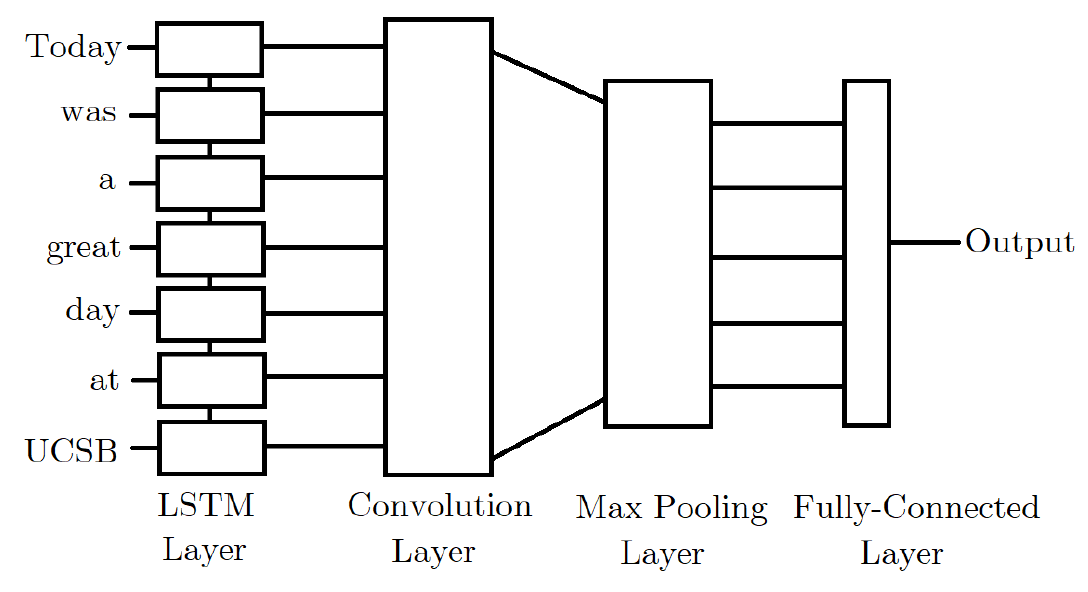
\includegraphics[width=\linewidth]{figure1.png}
  \caption{Sosa, P. (2017). LSTM-CNN Ensemble Model}
  \label{fig:fig1}
\end{figure}

The LSTM-CNN ensemble algorithm works as follows:
\begin{enumerate}
	\item The input Tweets are placed into [good, bad]-train.csv and [good, bad]-validation.csv for training and validation, respectively, where \textquotedblleft{}good\textquotedblright{} means the Tweet has positive sentiment and \textquotedblleft{}bad\textquotedblright{} means the Tweet has negative sentiment. Each line of the csv file contains the text of a Tweet.
	\item The code reads in the training and validation datasets and adds the label \textquotedblleft{}1.0\textquotedblright{} for positive Tweets and \textquotedblleft{}0.0\textquotedblright{} for negative Tweets.
	\item Since neural network models require input as numbers, each word in the entire dataset is assigned a unique integer ID and each Tweet string is transformed into a vector of these IDs. For example, if the dataset consists of \textquotedblleft{}I like dogs\textquotedblright{} and \textquotedblleft{}I like cats\textquotedblright{}, then the resulting vectors could be [0, 1, 2] and [0, 1, 3], respectively.
	\item For the training step, the dataset is split into equal-sized batches. The algorithm runs multiple passes/epochs through these batches. Each input Tweet in a batch will run through four layers of the LSTM-CNN algorithm in sequence:
	\item The embedding layer encodes each word ID in the input to a dense vector of floats (default embedding size 32). This is a more efficient representation since similar words would have similar encodings.
	\item The LSTM layer (32 units) takes in the encodings from the embedding layer and produces a new encoding for each input by using memory of previously discovered patterns. An overview of the LSTM structure is shown in figure 2. The LSTM layer consists of an \textquotedblleft{}input gate\textquotedblright{} that controls the input of new information into memory, a \textquotedblleft{}forget gate\textquotedblright{} that how long information is retained in memory, and a \textquotedblleft{}output gate\textquotedblright{} that controls how much the values stored in memory affect the output (Sosa 2017). The main benefit of having the LSTM layer is that it can potentially recognize sentence structures with changing sentiment, such as \textquotedblleft{}I hated programming until I took an AI course\textquotedblright{}. 
	\item The CNN layer takes the encodings from the LSTM layer and aims to learn local features. An overview of the CNN layer is shown in figure 3. The CNN layer extracts local features by applying multiple filters (default size [3, 4, 5]) on non-overlapping sections of the text. For example, a filter of size 3 applied on text \textquotedblleft{}I like CS and Math\textquotedblright{} may extract local features from the section \textquotedblleft{}CS and Math\textquotedblright{}. This may help the algorithm distinguish the sentiment in the usage of the word  \textquotedblleft{}bad\textquotedblright{} in \textquotedblleft{}very bad\textquotedblright{} versus \textquotedblleft{}not bad\textquotedblright{} (Sosa 2017). The output is then sub-sampled using max-pooling to reduce the model's dependence on the specific position of words in the input vector. The first layer of the CNN is the input layer and has as many nodes as there are words in the Tweet. The second layer by default has 32 nodes, each of which correspond to a filter and is connected to the corresponding input nodes of the filter. The third/max-pooling layer has size 2. The final dropout layer, with a configurable dropout probability, reduces overfitting and improves the generalization of the model. The CNN uses the Adam algorithm (a variation of gradient descent), the cross-entropy loss function, and the ReLu activation function. The output of the CNN layer is a vector of sentiment predictions with weights.
	\item Finally, the fully-connected layer takes in the scores and weights from the CNN layer and computes the final sentiment label by performing a dot product of the score and weights vectors. 
\end{enumerate}

Sosa's (2017) implementation of the LSTM-CNN algorithm is suitable for this project for a number of reasons. Firstly, the code is modular and easy to understand. Secondly, there are many accessible parameters which are clearly laid out in the main parameter section. Some of those critical parameters that can be tuned are batch size, filter sizes, number of filters and l2 regularization lambda. This means modifications to model parameters used in data preparation, training and evaluation can be done more efficiently and precisely. Furthermore, each step of the training procedure during the training stage is clearly defined. The implementation also includes evaluation summaries for training loss and accuracy during the training process. A final summary is also included after the training, which helps to evaluate the overall precision of the algorithm.

The implementation timeline is as follows. Jian will work on fetching Covid-19 data and Diwen and Zihao will work on pre-processing the existing Kaggle data for one week. Then, the three of us will work as a group to fully understand Sosa's implementation and train models without tuning any parameters. For the last 2 weeks, each group member will tune separate sets of the model's parameters to maximize its accuracy, and the best-tuned model will be picked as the final product.

\begin{figure}
  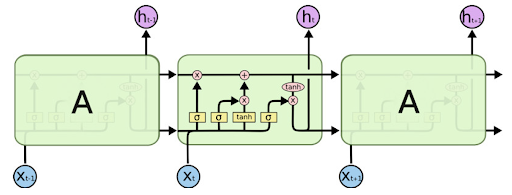
\includegraphics[width=\linewidth]{figure2.png}
  \caption{Sosa, P. (2017). LSTM Network Structure}
  \label{fig:fig2}
\end{figure}


\begin{figure}
  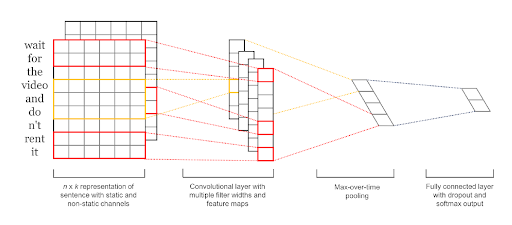
\includegraphics[width=\linewidth]{figure3.png}
  \caption{Kim, Y. (2014). Convolutional Neural Network for Sentence Classification}
  \label{fig:fig3}
\end{figure}


%%%%%%%%% Results %%%%%%%%%

\section{Results}

In Sosa's (2017) paper, the LSTM-CNN model trained and evaluated on generic Tweet datasets scored a 75.2\% accuracy. Without parameter tuning, it is expected that the initial accuracy of the LSTM-CNN model trained using a generic set of Tweets and evaluated on a Covid-19 dataset would be worse than 75.2\%. This is because Covid-19 Tweets are expected to have overwhelmingly negative sentiment and contain a highly skewed distribution of words and phrases when compared to a generic set of Tweets. With parameter tuning, it is expected that there will be a noticeable increase in accuracy as the model begins to learn more complex words, phrases and sentence structures.

%%%%%%%%% Bibliography %%%%%%%%%
\newpage
\nocite{*}
\bibliographystyle{aaai}
\bibliography{report}

\end{document}
